\subsubsection{Benchmark 1: Fibonacci Loop}
\begin{figure}[h]
\centering
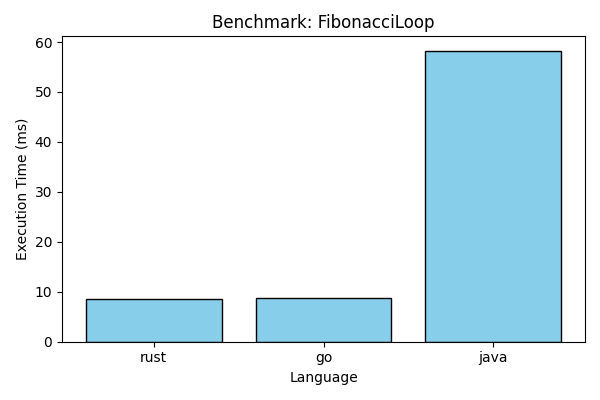
\includegraphics[width=\linewidth]{../Benchmark/Compute/FibonacciLoop/benchmark_FibonacciLoop.pdf}
\caption{Iterative Fibonacci computation: Rust vs Go vs Java}
\label{fig:fibonacci-benchmark}
\end{figure}
Rust and Go completed in under 9 ms, whereas Java took nearly 58 ms, motivating its removal from further analysis.


\subsubsection{Benchmark 2: Pi Computation}
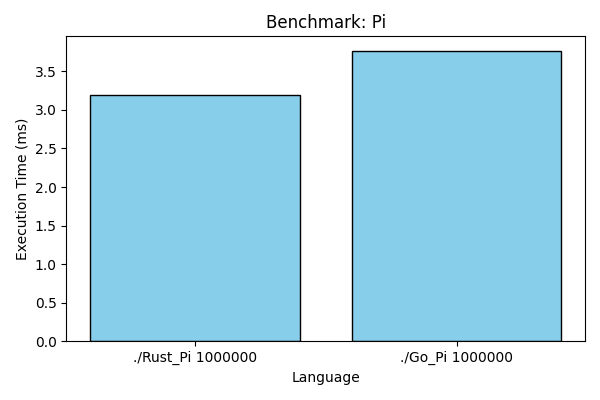
\includegraphics[width=\linewidth]{../Benchmark/Compute/Pi/benchmark_Pi.pdf}
\captionof{figure}{Execution time for Pi computation (1,000,000 iterations)}
\begin{figure}[h]
\centering
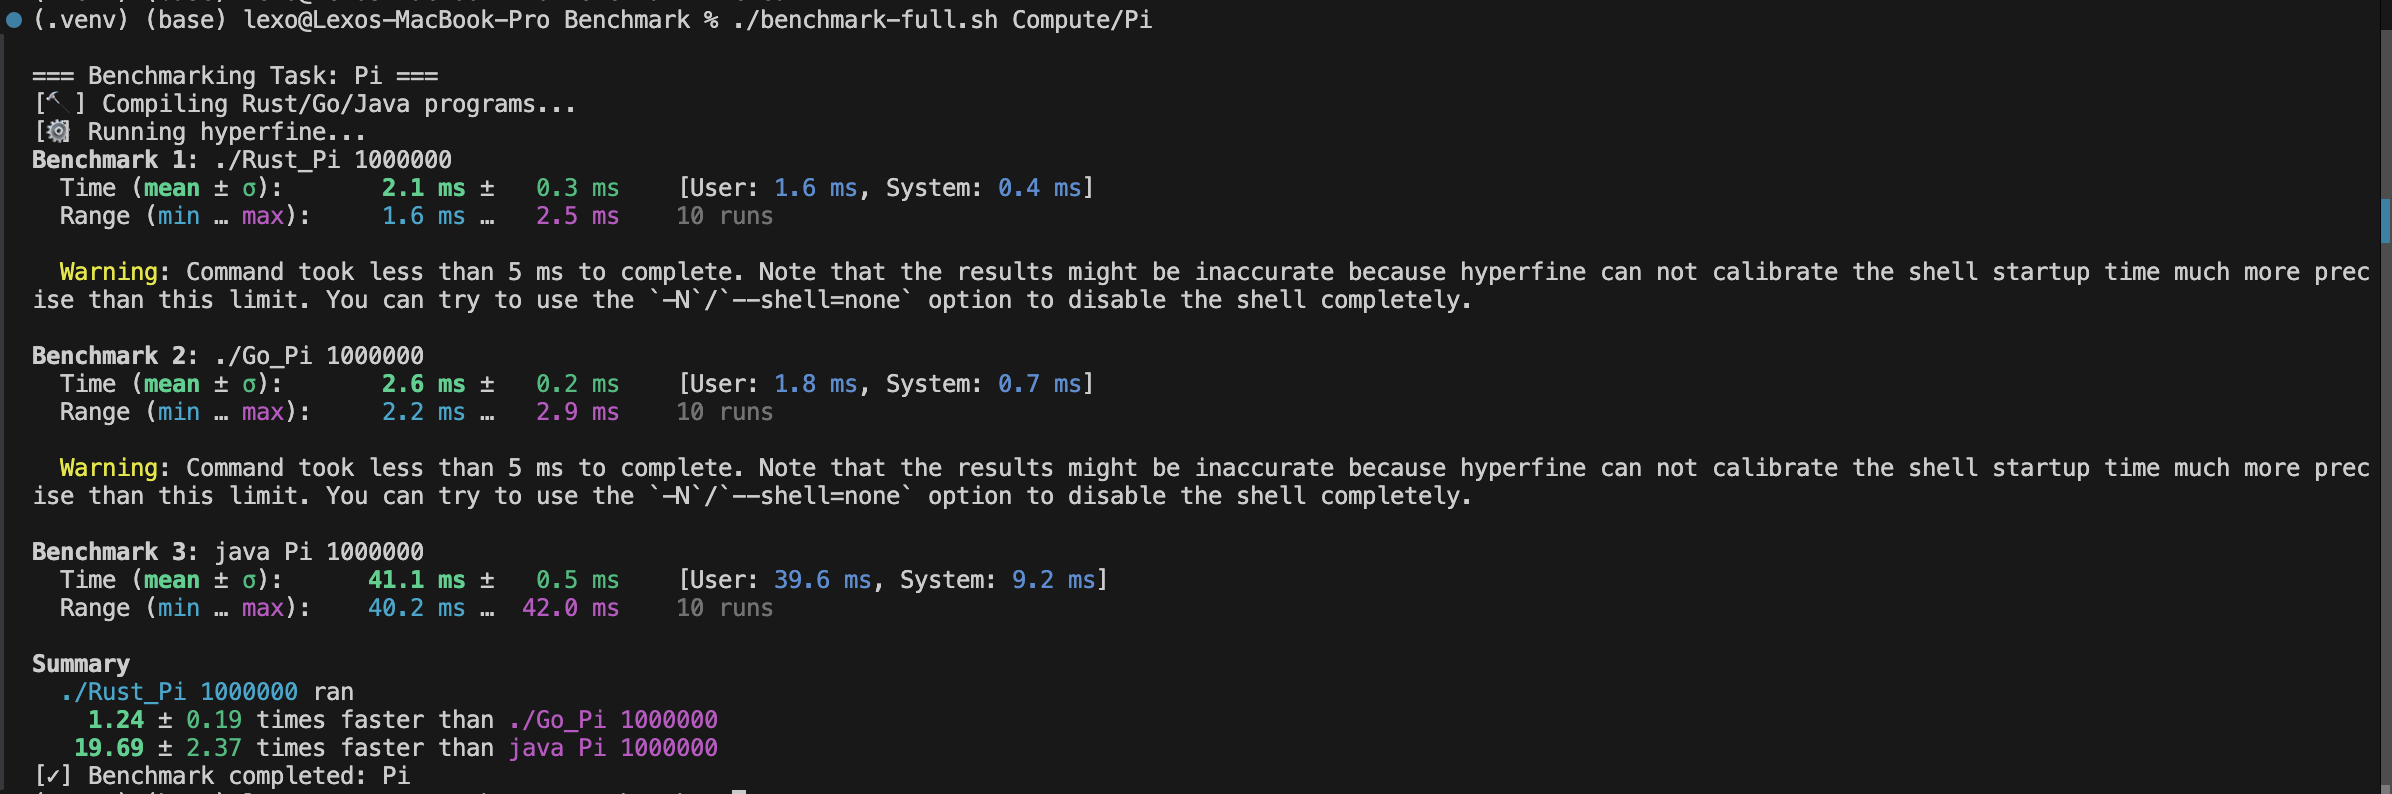
\includegraphics[width=0.9\linewidth]{./Pi_Result_Command_Line.png}
\caption{Performance comparison of Rust, Go, and Java on compute-bound task (π approximation)}
\label{fig:pi-benchmark}
\end{figure}
Rust completed the task in 2.1 ms and Go in 2.6 ms. Despite Rust's use of LLVM and manual memory, Go's GC overhead remained negligible in this compute-heavy task.

\subsubsection{Benchmark 3: Recursive Fibonacci}
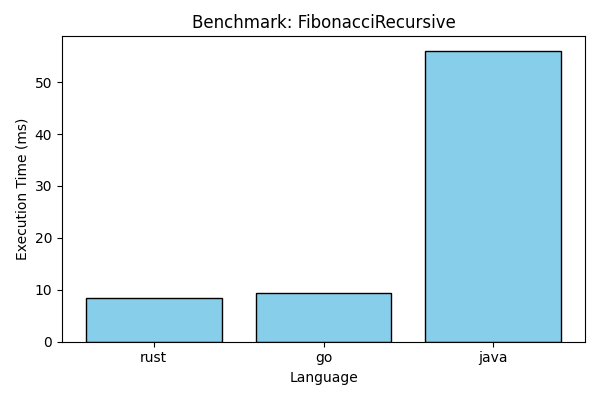
\includegraphics[width=\linewidth]{../Benchmark/Compute/FibonacciRecursive/benchmark_FibonacciRecursive.pdf}
\captionof{figure}{Recursive Fibonacci: Rust vs Go vs Java}
Again, Rust and Go performed closely (within 1 ms), showing consistent parity in CPU-bound workloads.

\subsubsection{Findings Summary}
These results challenge assumptions that garbage collection inherently causes significant slowdowns. In compute-dense workloads with minimal heap allocation, Go performs nearly as well as Rust.
